% Type de document
\documentclass[a4paper,12pt]{report}
 

% Chargement des extensions
\usepackage[utf8]{inputenc}
\usepackage[francais]{babel}
\usepackage{graphicx}
\usepackage[T1]{fontenc}
\usepackage{layout}
\usepackage{Garamond}

\begin{document}
\begin{titlepage}
\center
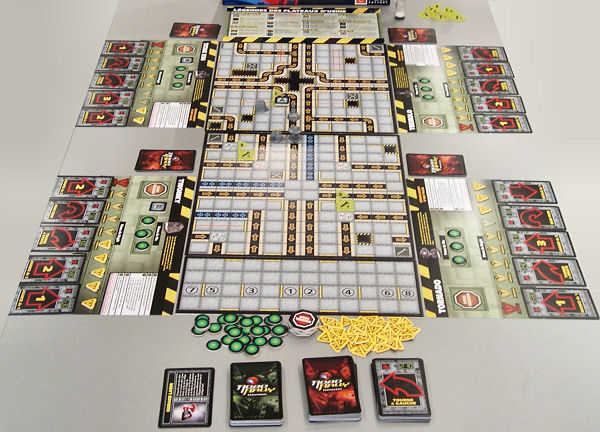
\includegraphics[width=0.8\textwidth]{Images/RoborallyPPage}\par\vspace{1cm}
	{\scshape\LARGE ENSTA Bretagne \par}
	\vspace{1cm}
	{\scshape\huge Projet informatique \par}
	\vspace{1cm}
	{\large\bfseries Rapport intermédiaire\par}
	\vspace{1cm}
	{\Large\itshape Romain DUSSOT et Thomas LE MASSON \par}

	\vfill
	{\large \today\par}
\end{titlepage}



% Debut du document



	\chapter*{Introduction}

Le sujet reprend le principe du jeu RoboRally, par le créateur du jeu de cartes Magic sorti en 1994 chez \textit{Wizard of the Coast}. Ce jeu se joue originellement de 2 à 8 joueurs. Dans notre cas le nombre de joueurs sera limité pour le moment. Les règles se trouvent aussi légèrement modifié. Nous allons commencer par parler rapidemment du jeu de société pour expliquer les règles de bases, ensuite nous detaillerons nos choix de conception.

    	\addcontentsline{toc}{chapter}{Introduction}

   	\chapter{Le jeu RoboRally, les règles}

	\section{Le but du jeu}

Le but du jeu est de rempoter la course définit sur le plateau. Pour ce faire, plusieurs moyens s'offrent \'a vous, comme:
\begin{itemize}
\item faire le trajet prédéterminé en passant par tous les checkpoints puis en finissant sur l'arrivée;
\item détruire vos adversaires en utilisant le plateau de jeu et ses fonctionnalités tels que les lasers.
\end{itemize}

	\section{Les cartes, les points de vie}

Un joueur dispose de 3 vies, donc son robot peut mourir 3 fois. Ce robot a 9 points de vies par vie. Ce qu'il lui permet d'encaisser 9 points de dégâts par vie. Ces points de vie représente également le nombre de cartes qu'il peut récupérer par tour. Le joueur récupère donc 9 cartes par tour de programmation.

	\section{Le déroulement}

		\subsection{La phase d'initialisation}

On choisit un parcours de jeu. Chaque joueur choisit un robot qui sera placé sur la plateau. 	Chaque joueur dispose de 3 vies et de 9 points par vie.

		\subsection{Les tours}

Un tour se décompose en 5 séquences immuables:
\begin{itemize}
\item On distribue les cartes programmes
\item On choisit les 5 cartes de programme de ce tour
\item On déclare ou si l'on se place \textit{hors tension} pour ce tour (possibilité expliquée juste après).
\item On joue dans l'ordre les cinq phases de programmation: exécution Programme, activation élèments de plateau, résolution les intéractions, enregistrement drapeau, réparation.
\item On prépare le tour suivant
\end{itemize}

		\subsection{La fin}

Le jeu se finit par plusieurs cas de figures:
\begin{itemize}
\item l'arrêt d'un des joueurs sur la case d'arrivée en étant passer par tous les checkpoints;
\item le destruction et la perte de tous les points de vie de tous les joueurs sauf un.
\end{itemize}
   	\section{Le plateau}

Le plateau dispose de plusieurs cases avec des fonctions bien précises.

\begin{figure}[!ht]
\center
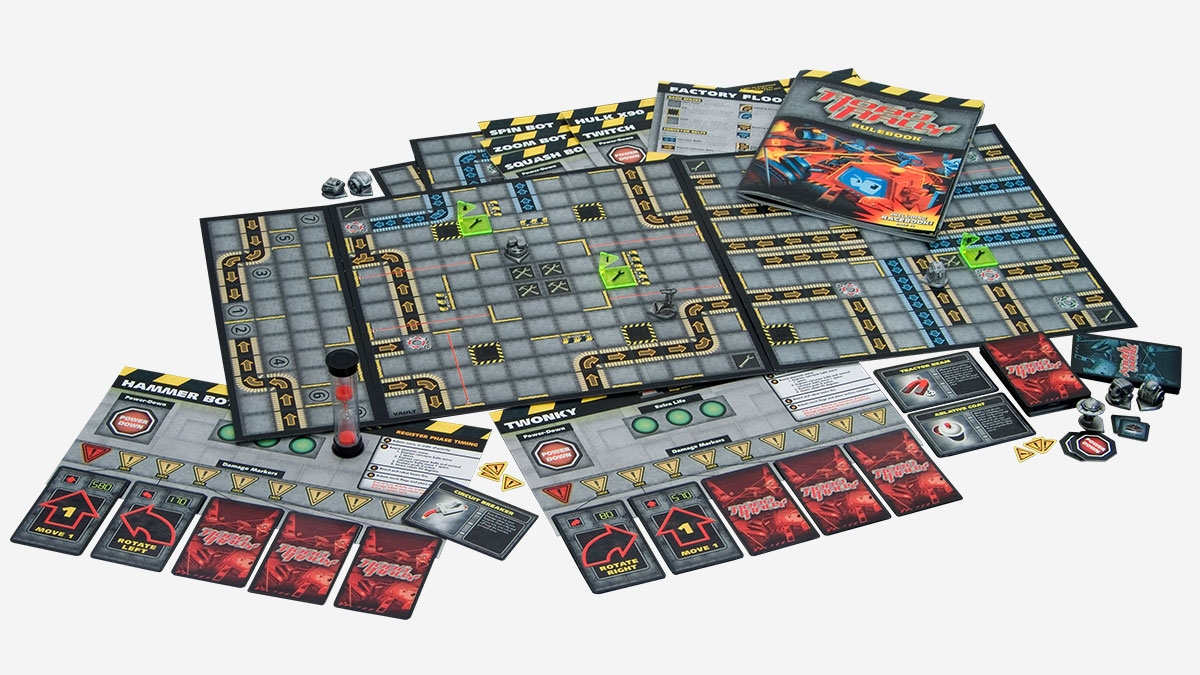
\includegraphics[scale = 0.3]{Images/plateau}
\caption{Plateau de jeu}

\end{figure}

    		\subsection{Les cases simples}

Les cases simples n'ont pas d'action sur les robots présents sur le plateau. Celles-ci sont construites à partir du sol et des murs qui y sont liés.On trouve donc 4 murs possibles sur la case, qui empêchent les robots de traverser et qui peuvent permettre de stopper sa course. La direction ou l'emplacement des robots ne sont modifiés par ces cases.

 		\subsection{Les cases munies de laser}

Sur certaines cases, on va pouvoir trouver des lasers qui vont infliger 1 points de dégâts au robot sur sa route. Les lasers ne peuvent être arrêté que par un mur. Ceux-ci se manifestent à chaque étapes de tour.

		\subsection{Les cases agissant sur les robots}
		
			\paragraph{Les giratoires}
			
Ces cases font tourner les robots à chaque étape. Elles modifient la situation actuelle. Le sens de rotation est défini selon le type de giratoire (à droite ou à gauche). Le graphisme de ses cases permet de voir directement le sens de rotation assigné à la case.

			\paragraph{Les tapis roulants}
			
Les tapis roulants peuvent ou non agir sur la directioin principale du robot, mais leur principal action est de faire translater le robot de 1 ou 2 cases selon le tapis. Comme les giratoires, ces cases agissent à toutes les étapes. 

			\paragraph{Jouer avec ses éléments}
			
Ces éléments étant assez complexe à utiliser car il modifie la sitation. Nous n'en prendrons pas compte au début de notre projet, nous nous interreserons au fait de les ajouter plus tard.



	\chapter{Notre travail}

	\section{Définition des classes}

Dans un premier temps, nous avons choisi de faire la distinction entre les cartes, les robots et les joueurs, en les définissants dans des classes différentes plus simple à créer. L' objectif étant d'utiliser des fonctions pour les faire interagir entre elles lors du déroulement du jeu.
Nous avons donc défini trois classes principales : les cartes, les robots et les joueurs. 

		\subsection{la classe "Carte"}
	
	Il existe dans ce jeu quatre types de cartes : « avancer », « reculer », « tourner » et « demi-tour ».
On peut avancer de une, deux ou trois cases. On peut reculer d'une case. On peut tourner d’un quart de tour vers la gauche ou vers la droite. On peut faire demi-tour.

Nous avons donc défini la classe « carte » avec quatre classes héritières.

Le constructeur de la classe « carte » est défini par quatre items :
\begin{itemize}
\item La priorité ;
\item Le nombre de rotation ;
\item Le nombre de case ;
\item Le numéro du joueur à laquelle elle appartient.  
\end{itemize}

Chacun des types de cartes est donc caractérisé par ces quatre items.

Les cartes de types « avancer » et « reculer » ont un nombre de rotation égale à zéro, les cartes « avancer » ont un nombre de case variant de 1 à 3 et la carte « reculer » a un nombre de case égale à -1.
Les cartes « tourner » ont un nombre de case égale à zéro, un nombre de rotation égale à 1 indique une rotation vers la droite et un nombre de rotation égale à -1 une rotation vers la gauche.
La carte « demi-tour » a un nombre de case nul et un nombre de rotation de 2.

		\subsection{la classe "Robot"}
	
Chaque joueur dispose d’un robot qu’il déplace à l’aide de ses cartes vers la ligne d’arrivée. Nous avons choisi de faire la distinction entre un joueur et son robot pour simplifier le programme et éviter de créer une classe trop complexe.


Le constructeur de la classe « robot » est défini par quatre items :

\begin{itemize}
\item La vie ;
\item La direction de départ ;
\item Les coordonnées ;
\item Le plateau : nous avons choisi de lier le robot au plateau afin de faciliter les mouvements de celui-ci au cours de la partie.
\end{itemize}

Le robot peut avancer, reculer et tourner. Nous avons décidé de créer des fonctions, au sein de la classe « robot », qui ont pour objectif de modifier les caractéristiques du robot en fonction de la carte jouée.

On a alors une fonction « Turn », qui modifie la direction du robot en prenant en entrer le nombre de rotations de la carte jouée. On a également une fonction « Forward », qui en prend en compte la direction du robot et fait évoluer les coordonnées du robot en fonction du nombre de case de la carte jouée.  	


		\subsection{la classe "Joueur"}


Chaque joueur a autant de carte dans sa main que de point de vie et est lié à son robot. Au début de la partie le joueur choisit un robot qui est placé aléatoirement sur le plateau de jeu.

Pour s’assurer que le vainqueur ait bien respecté les conditions de victoire en passant dans l’ordre par les différents check-points, nous avons créé dans le constructeur de la classe « joueur » un item « fil rouge » qui prend en compte cet aspect du jeu.

Le constructeur de la classe « joueur » est donc défini par quatre items :
\begin{itemize}
\item Le nombre dans la main du joueur ;
\item Le nombre de cartes jouées ;
\item Le robot ;
\item Le fil rouge, qui est une liste de 0/1 si les conditions de victoire sont vérifiées et déclenche la fin de la partie.
\end{itemize}

La classe « joueur » est également composée de deux sous classes : Utilisateur et IA, que nous n’avons pas encore définies.

		\subsection{Le plateau}
		
Pour définir le plateau de manière la plus simple pour nous. Nous avons décidé d'utiliser un dictionnaire personnalisé qui nous permet de répertorier toutes les cases existantes et de leur attribuer un caractère. Ensuite, grâce à la lecture de fichier texte incluse dans python, nous allons seulement lire notre fichier texte. Un exemple sera plus parlant:


\begin{figure}
\center
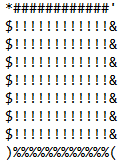
\includegraphics{Images/ImagePlateau}
\caption{Comment écrire un plateau en format texte}
\end{figure}

\begin{figure}
\center
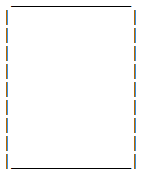
\includegraphics{Images/ImagePlateauReel}
\caption{Aperçu du plateau généré}
\end{figure}

\newpage
	\section{Diagramme des classes récapitulatif}
	
\begin{figure}[!ht]
\center
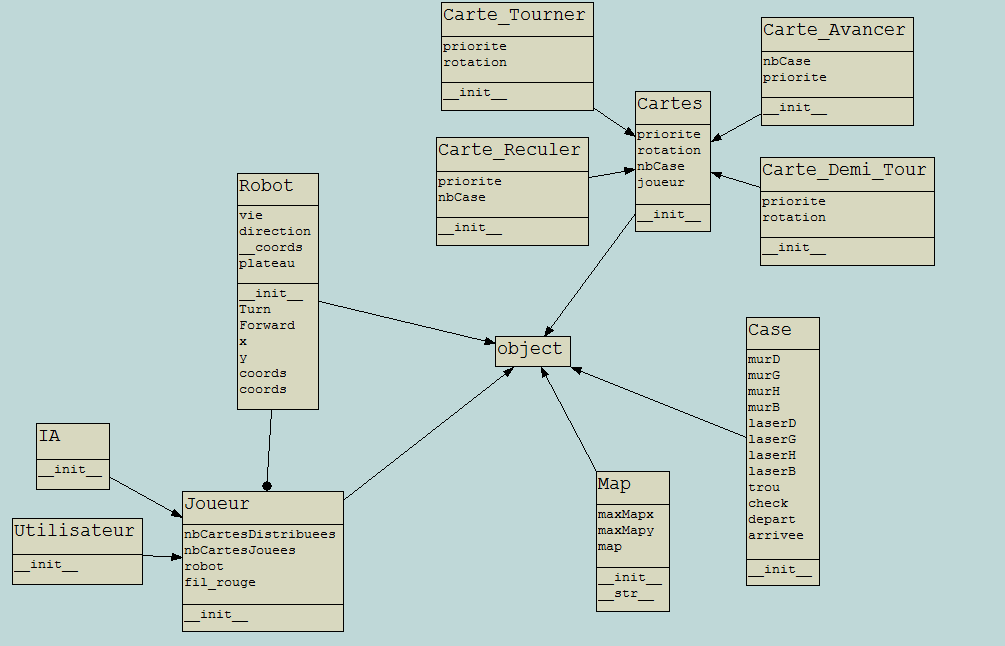
\includegraphics[scale = 0.6]{Images/DiagClasse}
\caption{Diagramme des classes}

\end{figure}	

	\section{Déroulement du jeu en vue de la programmation}

		\subsection{Initialisation}

La fonction initialisation remplit ce rôle en prenant en entrée le nombre d’IA et le nombre de joueur. Elle attribue à chaque joueur et à chaque IA son numéro de joueur et crée deux listes « Bot » et « Joueur » où elle les range. Elle charge également le plateau.

		\subsection{Les tours}

La phase de distribution est décrite par une fonction « Distribution ». Cette fonction attribue aléatoirement à chaque joueur autant de carte que son nombre de point de vie et crée la relation d’appartenance d’une carte à son joueur. Les cartes distribuées sont rangées dans des listes qui représentent les mains de chacun des joueurs.

La phase de choix est une phase d’interaction où l’utilisateur va entrer une liste ordonnée des 5 cartes qu’il veut jouer lors de ce tour. Nous n’avons pas encore défini la fonction liée à l’IA qui sera responsable du choix des cartes.

La phase d’application est composée de deux fonctions : une fonction de tri, qui trie une liste par ordre de priorité de chaque carte. Ensuite la fonction « Application des cartes prend la première carte de chaque joueur pour les mettre dans une liste, qui est ensuite triée par la fonction de tri. La liste triée est parcourue et toute les cartes sont appliquées une à une. Cette séquence est réalisée dans une boucle qui est réalisée 5 fois. 

	
% Fin du document
\end{document}